\documentclass[11pt,a4paper]{article}
\usepackage[a4paper,left=22mm,right=22mm,bottom=22mm,top=22mm]{geometry}
\usepackage{fontspec}
\usepackage[british]{babel}
\usepackage{amsmath,amssymb,graphicx,booktabs,array,tabularx,fancyhdr,multirow}
\usepackage[square,comma,numbers,sort&compress]{natbib}
\usepackage[hidelinks]{hyperref}
\usepackage{caption,subcaption}
\usepackage{microtype}
\usepackage{xcolor}
\graphicspath{{figures/}}
\captionsetup{font=small,labelfont=bf}
\setlength{\parindent}{0em}
\setlength{\parskip}{0.4em}
\setlength{\headheight}{14pt}
\renewcommand{\topfraction}{0.9}
\renewcommand{\textfraction}{0.07}
\renewcommand{\floatpagefraction}{0.8}
\pagestyle{fancy}
\fancyhead{}
\fancyhead[C]{\small Lab 5: Feature tracking and matching}
\fancyfoot{}
\fancyfoot[C]{\thepage}
\renewcommand{\headrulewidth}{0pt}
\renewcommand{\abstractname}{Summary}
\newcommand{\studentname}{Team Fullcans}
% Monospace identifiers may break after underscores and dots.
\DeclareRobustCommand{\code}[1]{\begingroup\ttfamily\codebreaks#1\endgroup}
\newcommand{\codebreaks}{\renewcommand{\_}{\textunderscore\allowbreak}}
\setlength{\emergencystretch}{3em}
\title{Lab 5 Report\\[0.3em]\large Feature detection, description, matching and tracking}
\author{\studentname}
\date{Report date: 23 October 2026}
\hypersetup{pdftitle={Lab 5 Report: Feature tracking and matching}}

\begin{document}
\maketitle

\begin{abstract}
We implemented the Lab~5 stencil (ROS Noetic, OpenCV~3.4.2 + contrib built by the
official \code{opencv3\_catkin} package): SIFT, SURF, ORB and FAST+BRIEF trackers with
$k$NN matching, Lowe's ratio test and RANSAC inlier detection; a Harris + pyramidal
Lucas--Kanade tracker; and Farneback dense optical flow. On the \code{box} image pair
SIFT reproduces the handout (603/969 keypoints, 79 inliers, 79\,\% inlier ratio) and
SURF gives the most inliers (88), while ORB only works once the scale pyramid is
enabled. On the two video datasets all methods have $>84\,\%$ inlier ratio;
Harris+LK is the most reliable (95--99.7\,\% inliers) and, together with FAST+BRIEF, the
fastest (3.0--5.9\,ms per frame pair), ORB is the best descriptor-based compromise, and
SIFT is 12--33$\times$ slower than those two. Section~\ref{sec:team} lists the commands that reproduce
every number in this report.
\end{abstract}


\section{Individual work}

Throughout this section the camera has principal point $(0,0)$, focal length $1$,
$s_x=s_y=1$ and $s_\theta=0$, so a point $p=[x\ y\ z]^\top$ with $z>0$ projects to
$(u,v)=(x/z,\,y/z)$, and the pixel $(u,v)$ corresponds to the ray of points
$\lambda w$, $\lambda>0$, with $w=[u\ v\ 1]^\top$.

\subsection{Deliverable 1 -- Perspective projection of a sphere}

\paragraph{1. Sphere on the optical axis.}
Let the centre be $c=[0\ 0\ d]^\top$. Because $d>r+1$, the whole sphere lies in front
of the image plane $z=1$ (every point has $z\ge d-r>1$), so it is entirely visible.
A pixel $(u,v)$ belongs to the image of the sphere iff its ray $\{\lambda w\}$ meets the
sphere, i.e.\ iff the distance from $c$ to the line through the origin with direction
$w$ is at most $r$:
\begin{equation}
  \frac{\lVert c\times w\rVert^2}{\lVert w\rVert^2}\le r^2 .
\end{equation}
The boundary of the image (the \emph{occluding contour}) is formed by the rays tangent
to the sphere, where equality holds. With $c\times w=[-dv\ \ du\ \ 0]^\top$,
$\lVert c\times w\rVert^2=d^2(u^2+v^2)$ and $\lVert w\rVert^2=u^2+v^2+1$, hence
\begin{equation}
  d^2(u^2+v^2)=r^2(u^2+v^2+1)
  \quad\Longleftrightarrow\quad
  \boxed{\,u^2+v^2=\frac{r^2}{d^2-r^2}\,}.
\end{equation}
The projection is a disc centred at the principal point whose boundary is a circle of
radius $\rho=r/\sqrt{d^2-r^2}$ (well defined since $d>r$).
Geometrically, the tangent rays form a right circular cone with apex at the optical
centre, axis along the optical axis and half-angle $\alpha$ with $\sin\alpha=r/d$; the
image plane is perpendicular to the axis, so it cuts the cone in a circle of radius
$\tan\alpha=r/\sqrt{d^2-r^2}$. For $d\gg r$ this tends to $r/d$, the familiar
``size divided by depth'' rule.

\paragraph{2. Sphere at an arbitrary position.}
For a general centre $c=[c_x\ c_y\ c_z]^\top$ the tangency condition
$\lVert c\times w\rVert^2=r^2\lVert w\rVert^2$ can be rewritten with
$\lVert c\times w\rVert^2=\lVert c\rVert^2\lVert w\rVert^2-(c^\top w)^2$ as
\begin{equation}
  (c_x u+c_y v+c_z)^2=k\,(u^2+v^2+1),\qquad k=\lVert c\rVert^2-r^2 .
  \label{eq:conic}
\end{equation}
This is a quadratic equation in $(u,v)$, so the contour is always a \textbf{conic}: the
intersection of the tangent cone (still a right circular cone, but now with its axis
along $c$) with the image plane, which is no longer perpendicular to the axis.
Rotating the image axes so that $u'$ points along $(c_x,c_y)$ and writing
$\rho_c=\sqrt{c_x^2+c_y^2}$, \eqref{eq:conic} becomes, after completing the square,
\begin{equation}
  (c_z^2-r^2)\Bigl(u'-\frac{\rho_c c_z}{c_z^2-r^2}\Bigr)^2+k\,v'^2=\frac{r^2k}{c_z^2-r^2}.
\end{equation}
\begin{itemize}
  \item If the sphere is fully in front of the camera ($c_z>r$, hence $k>0$) both
    coefficients are positive: the projection is an \textbf{ellipse} centred at
    $u'_0=\rho_c c_z/(c_z^2-r^2)$, $v'_0=0$, with semi-axes
    \[a_{\text{radial}}=\frac{r\sqrt{\lVert c\rVert^2-r^2}}{c_z^2-r^2},\qquad
      a_{\perp}=\frac{r}{\sqrt{c_z^2-r^2}} .\]
    The major axis points radially away from the principal point and the elongation
    $a_{\text{radial}}/a_\perp=\sqrt{(\lVert c\rVert^2-r^2)/(c_z^2-r^2)}\ge 1$ grows
    as the sphere moves towards the border of the field of view. Note that the centre of
    the ellipse is \emph{not} the projection $\rho_c/c_z$ of the sphere centre; it is
    shifted outwards. For $c_x=c_y=0$ we recover the circle of part 1.
  \item If the sphere touches the plane $z=0$ through the optical centre ($c_z=r$) the
    $u'^2$ coefficient vanishes and the contour is a \textbf{parabola}; if it crosses
    that plane ($|c_z|<r$, camera still outside the sphere) the coefficients have
    opposite signs and the contour is (one branch of) a \textbf{hyperbola}. These cases
    are only of theoretical interest because part of the sphere is behind the camera.
\end{itemize}

\subsection{Deliverable 2 -- Vanishing points}

\paragraph{1. Vanishing point of a family of parallel lines.}
Write a 3D line as $p(\lambda)=p_0+\lambda u$ with $\lVert u\rVert=1$. Its image is
\begin{equation}
  \pi(p(\lambda))=\Bigl(\frac{p_{0,x}+\lambda u_x}{p_{0,z}+\lambda u_z},\
                        \frac{p_{0,y}+\lambda u_y}{p_{0,z}+\lambda u_z}\Bigr).
\end{equation}
If $u_z\neq0$, letting $\lambda\to\infty$ (the direction in which the line moves away
from the camera, i.e.\ $\lambda u_z>0$) gives
\begin{equation}
  \boxed{\,v_\infty=\Bigl(\frac{u_x}{u_z},\ \frac{u_y}{u_z}\Bigr)\,}
\end{equation}
which depends only on the direction $u$ and not on the point $p_0$. Hence every line
with direction $u$ -- in particular two parallel lines $p_0+\lambda u$ and
$q_0+\mu u$ -- passes through $v_\infty$ in the image: $v_\infty$ is the vanishing
point. It is the image of the point at infinity $[u^\top\ 0]^\top$, i.e.\ the
intersection of the image plane with the ray through the optical centre parallel to the
lines. With a general calibration matrix $K$ it reads $v_\infty\simeq Ku$ in homogeneous
coordinates.

\emph{Geometric view.} Each 3D line together with the optical centre $O$ spans a plane
whose intersection with the image plane is the image line. For two parallel lines both
planes contain the direction $u$, so they intersect along the line through $O$ with
direction $u$; this line hits the image plane exactly at $v_\infty$.

\paragraph{2. When do parallel lines stay parallel?}
\textbf{Claim:} the images of two (distinct, not through $O$) parallel 3D lines are
parallel if and only if their direction is parallel to the image plane, $u_z=0$.

\emph{Proof.} ($\Leftarrow$) If $u_z=0$ the depth along the line is constant,
$z=p_{0,z}$, and
$\pi(p(\lambda))=\frac{1}{p_{0,z}}[p_{0,x}\ p_{0,y}]^\top+\frac{\lambda}{p_{0,z}}[u_x\ u_y]^\top$:
the image is a line with direction $[u_x\ u_y]^\top$. The second line has the same image
direction, so both image lines are parallel (the vanishing point is at infinity,
$Ku$ has third coordinate $0$).
($\Rightarrow$) If $u_z\neq0$ both image lines contain the finite point $v_\infty$ from
part 1, so they intersect there and cannot be parallel (they can only coincide, when
the two 3D lines are coplanar with $O$). $\square$

In the geometric picture: the two planes through $O$ meet in the line through $O$ with
direction $u$; this line meets the image plane at a finite point unless it is parallel to
it, i.e.\ $u_z=0$. A practical consequence is that, for a camera looking straight at a
wall, the horizontal and vertical edges on the wall stay parallel in the image, while
edges going in depth converge.


\section{Team work}\label{sec:team}

\subsection{Implementation and setup}

\paragraph{Build.} The official 2023 ROS1 stencil (\code{feature\_tracking}, package
\code{lab\_5}) is built in a catkin workspace together with \code{opencv3\_catkin}
(OpenCV 3.4.2 + contrib, which still contains the patented SIFT and SURF in
\code{xfeatures2d}). Compared with the official package we only switched off modules the
lab does not use (Python bindings, VTK/viz, FFMPEG) and replaced \code{glog\_catkin} by the
system glog. Because \code{cv\_bridge} exports the system OpenCV~4.2 libraries, we also
filter them out of the link line of \code{lab\_5}; otherwise two \code{highgui} versions
(GTK2 and GTK3) are loaded and \code{imshow} aborts. \code{scripts/build\_workspace.sh}
builds everything (OpenCV takes 4~min on 12
cores).

\paragraph{Descriptor-based trackers (D3--D6).} We compare SIFT~\cite{lowe2004sift},
SURF~\cite{bay2006surf}, ORB~\cite{rublee2011orb} and FAST~\cite{rosten2006fast} +
BRIEF~\cite{calonder2010brief}.
\code{FeatureTracker::trackFeatures} detects keypoints in both images
(\code{detector->detect}), describes them (\code{detector->compute}; for FAST the
descriptor is computed by a separate \code{BriefDescriptorExtractor}), and calls
\code{matchDescriptors}, which runs \code{knnMatch} with $k=2$ and keeps
\code{m[0]} if \code{m[0].distance < 0.8 m[1].distance} (matches with fewer than two
neighbours are dropped). SIFT and SURF use the default \code{FlannBasedMatcher}
(randomised kd-trees on float descriptors~\cite{muja2009flann}); ORB and BRIEF descriptors are binary, so they are
matched with a brute-force Hamming matcher (\code{BFMatcher(NORM\_HAMMING)}); a FLANN
LSH index is selectable with a parameter and compared below.
The good matches are passed to the provided \code{inlierMaskComputation}
(fundamental matrix with RANSAC, 3\,px epipolar threshold), and the inliers are drawn in
green over the red outliers with two \code{cv::drawMatches} calls
(\code{DRAW\_OVER\_OUTIMG}). All statistics are averaged by the provided code and also
logged per frame to CSV.

\paragraph{Two fixes to the stencil.} In video mode, \code{imageCallback} stored
\code{prev\_image = image}, where \code{image} comes from \code{cv\_bridge::toCvShare} and
does not own its pixels; we keep a \code{clone()} instead. The first frame was also
matched with itself (100\,\% inliers); it is now skipped.

\paragraph{Statistics.} As in the handout table, ``\# of Matches'' is the number of
$k$NN queries (one per keypoint of image~1), ``Good Matches'' are those that pass the
ratio test, and the inlier ratio is $\#\text{inliers}/\#\text{good matches}$. We added
the wall-clock time of detection + description + matching for one image pair (both images
are processed, drawing excluded; Intel Core i5-12400F, Release build).

\subsection{Deliverable 3 -- SIFT keypoints and descriptors}

Figure~\ref{fig:kp} shows the 603 and 969 SIFT keypoints detected in \code{box.png} and
\code{box\_in\_scene.png}, drawn with their scale (circle radius) and orientation.

\begin{figure}[h]
  \centering
  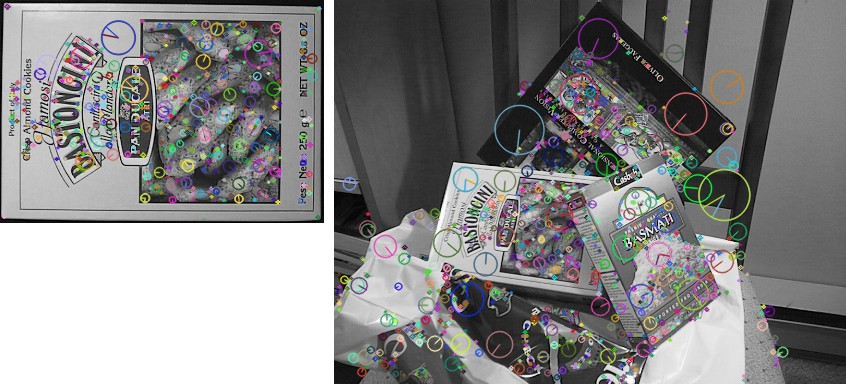
\includegraphics[width=\linewidth]{d3_sift_keypoints.jpg}
  \caption{SIFT keypoints (\code{DRAW\_RICH\_KEYPOINTS}): 603 in \code{box.png} (left),
    969 in \code{box\_in\_scene.png} (right).}
  \label{fig:kp}
\end{figure}

\subsection{Deliverable 4 -- Descriptor-based matching}

\begin{enumerate}
  \item The SIFT descriptor has \textbf{128 dimensions} (a $4\times4$ grid of 8-bin
    gradient orientation histograms), stored as \code{CV\_32F}: the descriptor matrices are
    $603\times128$ and $969\times128$.
  \item Figure~\ref{fig:matches}(a) shows the best FLANN match of every keypoint of
    \code{box.png} (603 matches). Most of them are wrong: every keypoint gets a nearest
    neighbour, even the ones on the background of \code{box.png} that do not exist in the
    second image.
  \item[3--4.] After the ratio test with threshold 0.8 only 98 matches remain
    (Fig.~\ref{fig:matches}(b)); almost all of them now connect the box to its copy in the
    scene, i.e.\ the ratio test removes most outliers. (FLANN's kd-trees are randomised,
    so the count varies between 95 and 104 over 20 runs, mean 99.7; the handout reports 93.)
\end{enumerate}

\begin{figure}[h]
  \centering
  \begin{subfigure}{0.49\linewidth}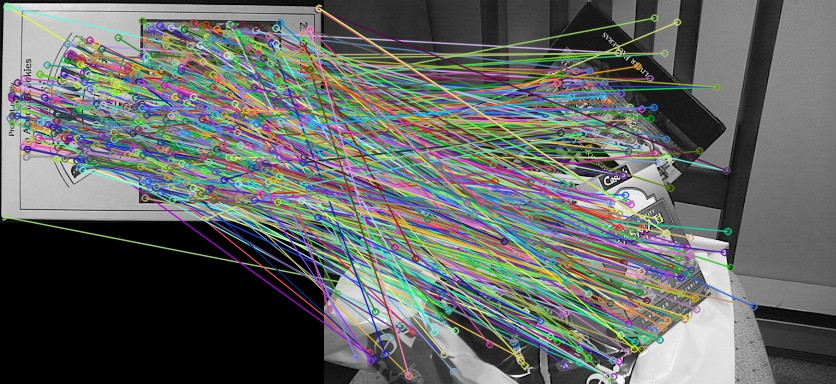
\includegraphics[width=\linewidth]{d4_sift_matches_all.jpg}
    \caption{All 603 nearest-neighbour matches.}\end{subfigure}\hfill
  \begin{subfigure}{0.49\linewidth}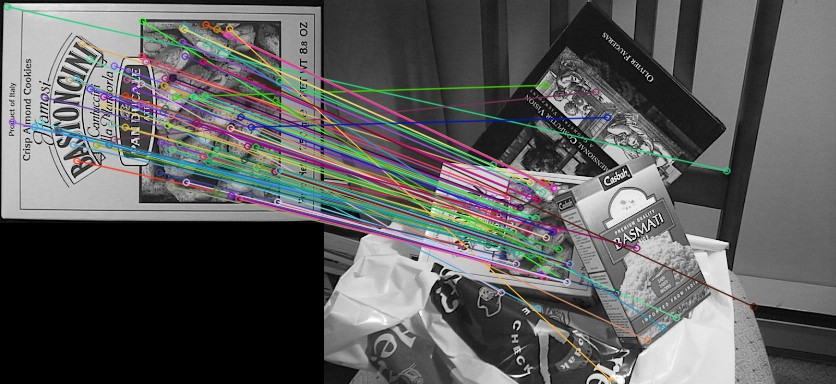
\includegraphics[width=\linewidth]{d4_sift_matches_ratio.jpg}
    \caption{98 matches after the ratio test.}\end{subfigure}
  \caption{SIFT + FLANN matches from \code{box.png} to \code{box\_in\_scene.png}.}
  \label{fig:matches}
\end{figure}

\subsection{Deliverable 5 -- Matching quality}

Figure~\ref{fig:inliers} shows the inliers (green) and outliers (red) of the 98 good
matches of that run; Table~\ref{tab:pair} (first column) gives the statistics averaged
over 20 runs, which agree with the handout (603 / 969 / 603 / 93 / 78 / 83.9\,\%).

\begin{figure}[h]
  \centering
  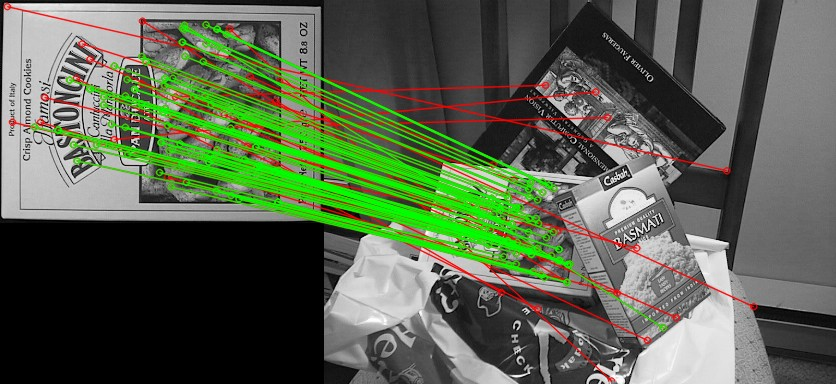
\includegraphics[width=0.75\linewidth]{d5_sift_inliers.jpg}
  \caption{SIFT: 76 RANSAC inliers (green) and 22 outliers (red) among the 98 ratio-test matches.}
  \label{fig:inliers}
\end{figure}

\subsection{Deliverable 6.a -- Comparison on the image pair}

\begin{table}[h]
  \centering
  \caption{Statistics on \code{box.png}$\to$\code{box\_in\_scene.png}. ORB: 2000
    features, 8 pyramid levels; FAST: threshold 10, 32-byte BRIEF; all others default.
    Mean of 20 runs (SIFT/SURF vary slightly because FLANN is randomised; the
    brute-force matches of ORB and BRIEF are deterministic).}
  \label{tab:pair}
  \begin{tabular}{lrrrr}
    \toprule
    Statistics & SIFT & SURF & ORB & FAST+BRIEF \\
    \midrule
\# of Keypoints in Img 1 & 603 & 997 & 1589 & 2266 \\
\# of Keypoints in Img 2 & 969 & 1822 & 1999 & 3653 \\
\# of Matches & 603 & 997 & 1589 & 2266 \\
\# of Good Matches & 100 & 137 & 73 & 41 \\
\# of Inliers & 79 & 88 & 55 & 17 \\
Inlier Ratio & 79.0\% & 64.2\% & 75.3\% & 41.5\% \\
Time / pair [ms] & 64.8 & 58.4 & 19.4 & 25.0 \\
    \bottomrule
  \end{tabular}
\end{table}

\paragraph{What we tried.} Table~\ref{tab:pairsweep} lists all configurations.
\begin{itemize}
  \item \textbf{ORB pyramid.} With the stencil's \code{ORB::create(500, 1.2, 1)} (one
    pyramid level, used to avoid the ``Unknown interpolation method'' error mentioned in
    the handout) ORB finds only 7 inliers, because the box appears about $2\times$
    smaller in the scene and ORB is then not scale invariant. With OpenCV~3.4.2 the
    8-level pyramid works without that error and gives 26 inliers (89.7\,\% ratio);
    raising the number of features to 2000 gives 55 inliers.
  \item \textbf{SURF Hessian threshold.} 100 (default) vs.\ 400: fewer keypoints and
    25\,\% faster, but 76 instead of 88 inliers. The default is kept.
  \item \textbf{FAST threshold.} 10 (default) vs.\ 30: fewer corners, but even fewer
    good matches. FAST+BRIEF is the weakest method on this pair: neither FAST nor BRIEF
    is scale invariant and BRIEF is not rotation invariant, and the box is both rotated
    and shrunk. Figure~\ref{fig:pairgrid} also shows that several of its 17 ``inliers''
    are visibly wrong: the fundamental-matrix test only checks the distance to an
    epipolar line, so with few correct matches RANSAC can accept wrong ones.
  \item \textbf{FLANN-LSH vs.\ brute force.} For ORB and BRIEF,
    \code{FlannBasedMatcher(new flann::LshIndexParams(20, 10, 2))} returns the same good
    matches as brute-force Hamming (we checked independently in Python that it returns the
    exact nearest neighbour for 498 of 500 ORB descriptors), but it is 5--20$\times$
    slower here because the LSH index is rebuilt for every image pair and the descriptor
    sets are small. Brute-force Hamming (XOR + popcount) is therefore the better choice.
\end{itemize}

\begin{table}[h]
  \centering\small
  \caption{All configurations tried on the image pair.}
  \label{tab:pairsweep}
  \begin{tabular}{llrrrrr}
    \toprule
    Method & Parameters & KP 1 & Good & Inliers & Ratio [\%] & ms \\
    \midrule
    SIFT & default & 603 & 100 & 79 & 79.0 & 64.8 \\
    SURF & Hessian 100 (default) & 997 & 137 & 88 & 64.2 & 58.4 \\
    SURF & Hessian 400 & 786 & 119 & 76 & 63.4 & 43.2 \\
    ORB & 500 feat., 1 level, BF (stencil) & 500 & 13 & 7 & 53.8 & 4.3 \\
    ORB & 500 feat., 1 level, FLANN-LSH & 500 & 13 & 7 & 53.8 & 20.7 \\
    ORB & 500 feat., 8 levels, BF & 453 & 29 & 26 & 89.7 & 8.8 \\
    ORB & 2000 feat., 8 levels, BF & 1589 & 73 & 55 & 75.3 & 19.4 \\
    FAST+BRIEF & threshold 10, BF & 2266 & 41 & 17 & 41.5 & 25.0 \\
    FAST+BRIEF & threshold 10, FLANN-LSH & 2266 & 41 & 17 & 41.5 & 476.6 \\
    FAST+BRIEF & threshold 30, BF & 1095 & 12 & 7 & 58.3 & 9.0 \\
    \bottomrule
  \end{tabular}
\end{table}

\begin{figure}[h]
  \centering
  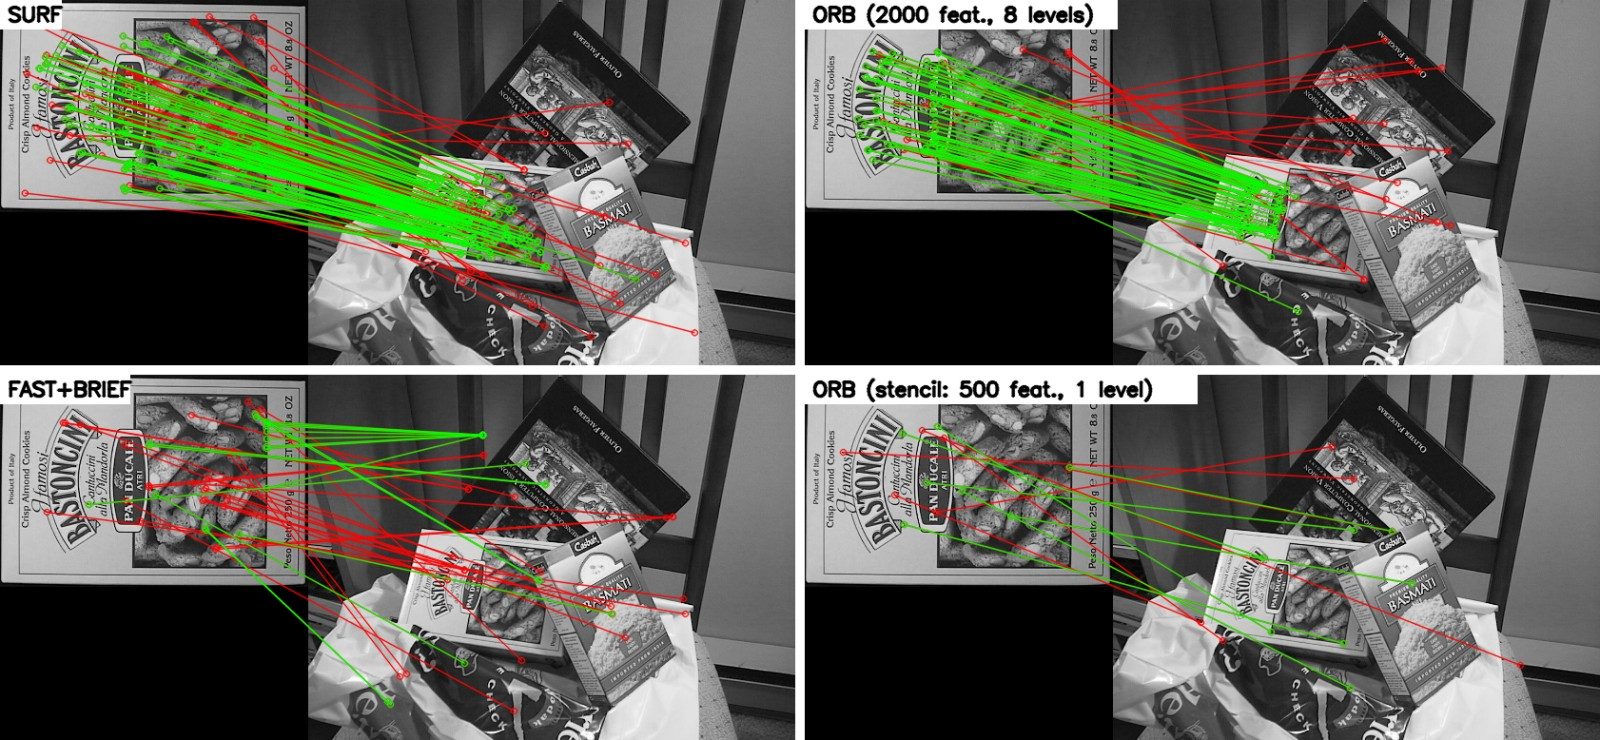
\includegraphics[width=\linewidth]{d6a_inliers_grid.jpg}
  \caption{Inliers (green) and outliers (red) for SURF, ORB (2000 features, 8 levels),
    FAST+BRIEF and the stencil ORB (500 features, 1 level).}
  \label{fig:pairgrid}
\end{figure}

\subsection{Deliverable 6.b -- Real datasets}

We used the two required bags:
\code{30fps\_424x240\_2018-10-01-18-35-06.bag} (real RealSense colour images,
$424\times240$, 1584 frames, a hand-held walk through a tunnel) and
\code{vnav-lab5-smooth-trajectory.bag} (simulated TESSE camera, $720\times480$, 1386
frames). Every consecutive pair of frames is matched (current frame = image~1, previous
frame = image~2). The bag is played at real-time rate; the subscriber queue (1000) is
large enough that no frame is dropped: 1578--1583 and 1382--1385 frame pairs were
processed (a few frames at the start/end of the bag are missed while the node connects or
shuts down). For every method we tried 2--3 parameter sets (Table~\ref{tab:videosweep})
and Tables~\ref{tab:30fps}--\ref{tab:smooth} use the one with the most inliers,
which was the same on both datasets.

\begin{table}[h]
  \centering
  \caption{Average over all frame pairs of \code{30fps\_424x240} (real data).}
  \label{tab:30fps}
  \begin{tabular}{lrrrrr}
    \toprule
    Statistics & SIFT & SURF & ORB & FAST+BRIEF & Harris+LK \\
    \midrule
\# of Keypoints in Img 1 & 741 & 467 & 923 & 828 & 561 \\
\# of Keypoints in Img 2 & 741 & 467 & 922 & 828 & 561 \\
\# of Matches & 741 & 467 & 923 & 828 & 561 \\
\# of Good Matches & 412 & 334 & 680 & 635 & 554 \\
\# of Inliers & 395 & 320 & 668 & 608 & 552 \\
Inlier Ratio & 94.6\% & 95.3\% & 98.1\% & 95.1\% & 99.7\% \\
Time / pair [ms] & 63.7 & 28.7 & 8.8 & 5.4 & 3.0 \\
    \bottomrule
  \end{tabular}
\end{table}

\begin{table}[h]
  \centering
  \caption{Average over all frame pairs of \code{vnav-lab5-smooth-trajectory} (simulated data).}
  \label{tab:smooth}
  \begin{tabular}{lrrrrr}
    \toprule
    Statistics & SIFT & SURF & ORB & FAST+BRIEF & Harris+LK \\
    \midrule
\# of Keypoints in Img 1 & 270 & 1194 & 787 & 568 & 276 \\
\# of Keypoints in Img 2 & 270 & 1192 & 786 & 568 & 276 \\
\# of Matches & 270 & 1194 & 787 & 568 & 276 \\
\# of Good Matches & 169 & 716 & 435 & 392 & 269 \\
\# of Inliers & 142 & 610 & 392 & 357 & 255 \\
Inlier Ratio & 84.4\% & 85.4\% & 89.9\% & 90.6\% & 95.5\% \\
Time / pair [ms] & 144.9 & 72.1 & 12.1 & 4.4 & 5.9 \\
    \bottomrule
  \end{tabular}
\end{table}

Parameters: SIFT contrast threshold 0.02 (default 0.04); SURF Hessian 100; ORB 2000
features, 8 levels; FAST threshold 10 + 32-byte BRIEF; ORB/BRIEF matched with
brute-force Hamming; ratio 0.8 everywhere. Harris+LK: up to 1000 corners, quality level
0.01, minimum distance 5\,px (Section~\ref{sec:lk}).

\begin{figure}[p]
  \centering
  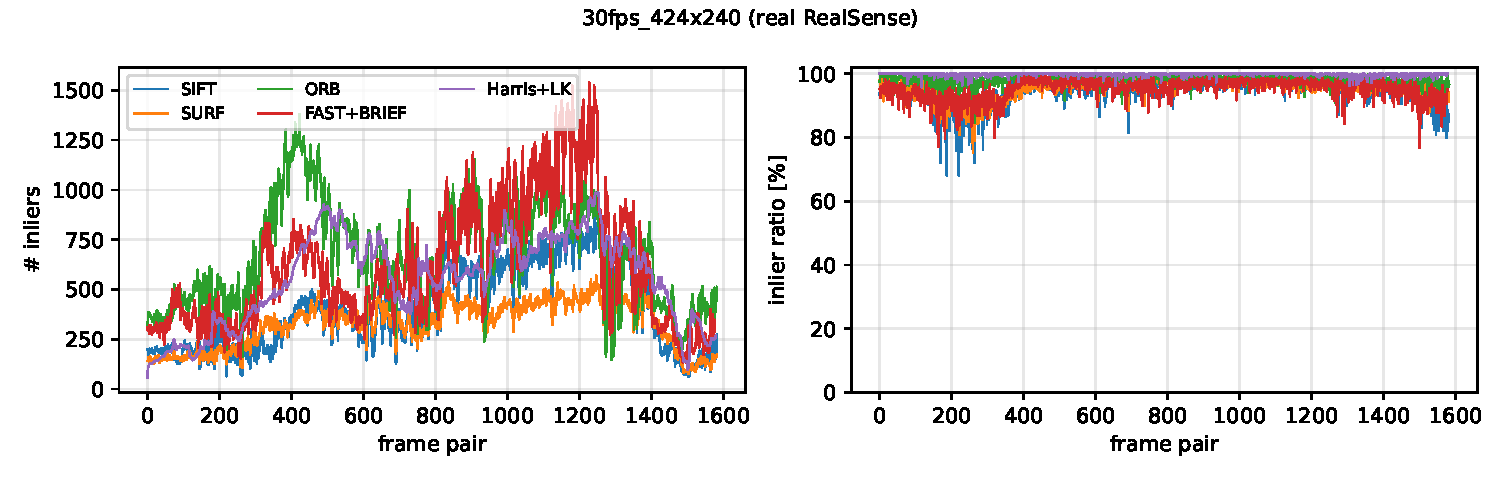
\includegraphics[width=\linewidth]{d6b_30fps_per_frame.pdf}\\[0.5em]
  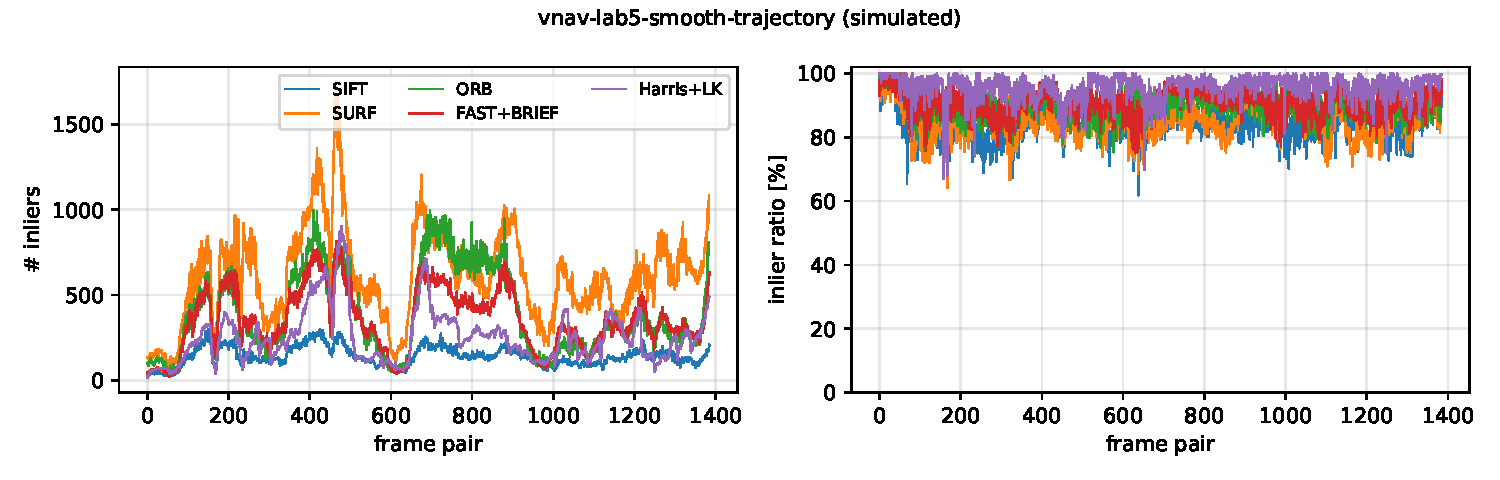
\includegraphics[width=\linewidth]{d6b_smooth_per_frame.pdf}
  \caption{Number of inliers and inlier ratio for every frame pair of the two datasets.}
  \label{fig:perframe}
\end{figure}

\begin{figure}[p]
  \centering
  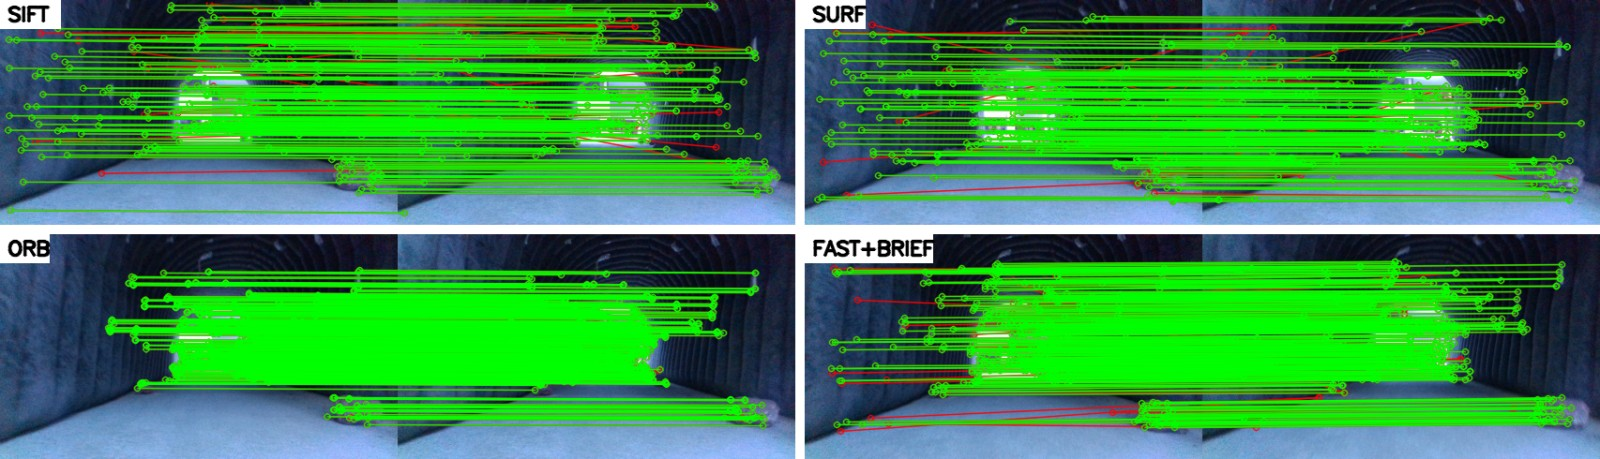
\includegraphics[width=\linewidth]{d6b_30fps_frame150.jpg}\\[0.5em]
  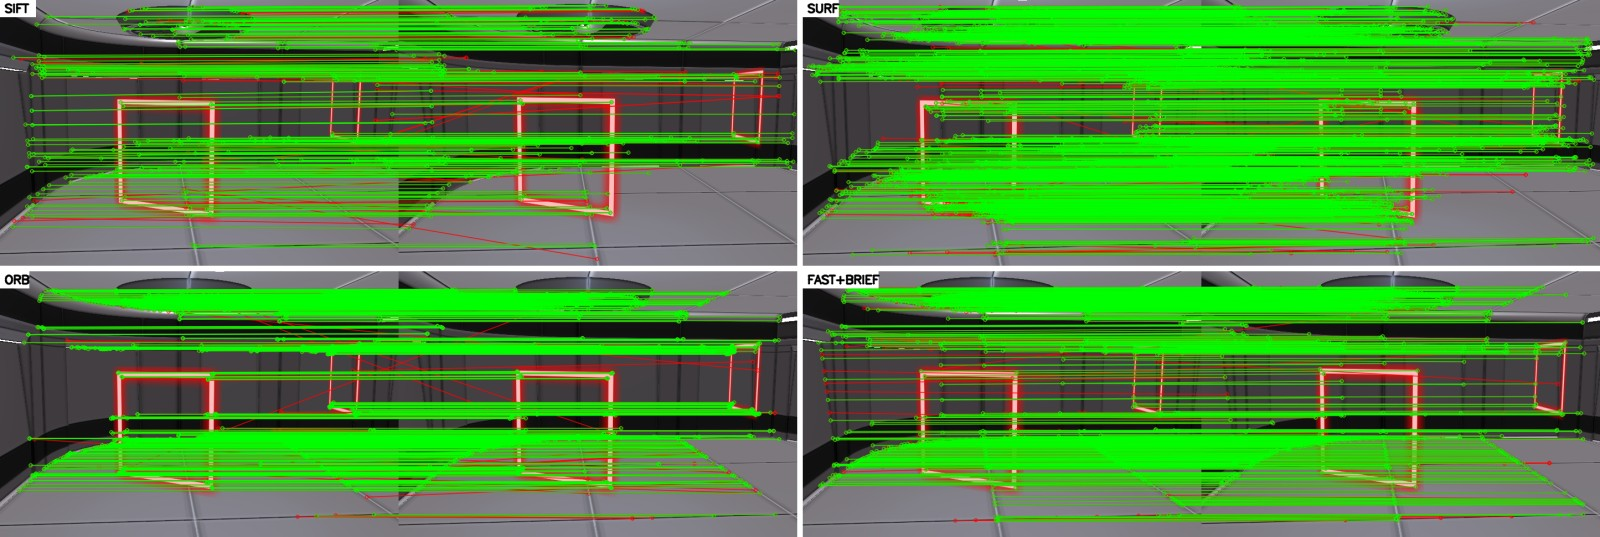
\includegraphics[width=\linewidth]{d6b_smooth_frame150.jpg}
  \caption{Inliers (green) and outliers (red) at frame pair 150 of each dataset (top:
    real, bottom: simulated). Full SIFT videos: \code{video/d6\_sift\_tracking\_*.mp4}.}
  \label{fig:videoframes}
\end{figure}

\begin{figure}[h]
  \centering
  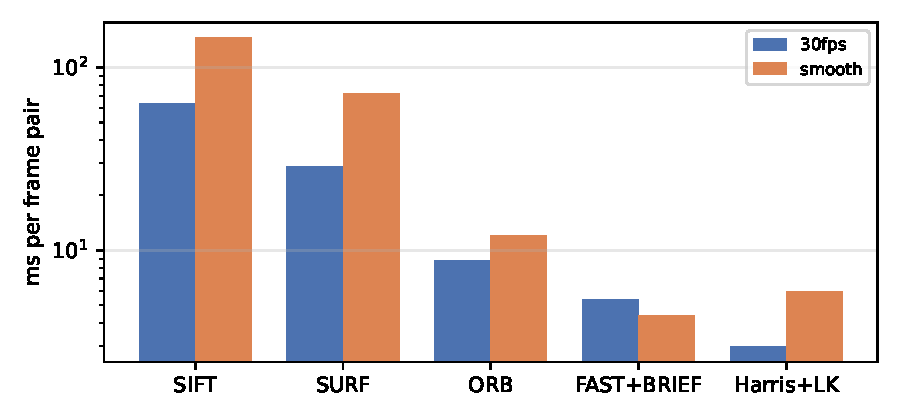
\includegraphics[width=0.65\linewidth]{d6b_timing.pdf}
  \caption{Average time per frame pair (detection and description of both frames +
    matching; for LK: tracking + re-detection). Log scale. Repeating the whole set of runs
    changed individual timings by up to $\pm30\,\%$ (system load), so only the order of
    magnitude and the ranking are meaningful; the counts changed by less than 1\,\%.}
  \label{fig:timing}
\end{figure}

\begin{table}[h]
  \centering\small
  \caption{All configurations tried on the videos (bold: used in Tables~\ref{tab:30fps}--\ref{tab:smooth}).}
  \label{tab:videosweep}
  \begin{tabular}{llrrrr@{\hspace{1.5em}}rrrr}
    \toprule
    & & \multicolumn{4}{c}{\code{30fps\_424x240}} & \multicolumn{4}{c}{\code{smooth-trajectory}} \\
    Method & Parameters & KP & Inl. & \% & ms & KP & Inl. & \% & ms \\
    \midrule
    SIFT & contrast 0.04 (default) & 404 & 249 & 95.7 & 64.1 & 148 & 81 & 86.4 & 131.8 \\
    \textbf{SIFT} & \textbf{contrast 0.02} & 741 & 395 & 94.6 & 63.7 & 270 & 142 & 84.4 & 144.9 \\
    \textbf{SURF} & \textbf{Hessian 100} & 467 & 320 & 95.3 & 28.7 & 1194 & 610 & 85.4 & 72.1 \\
    SURF & Hessian 400 & 266 & 200 & 97.0 & 16.4 & 476 & 260 & 87.3 & 41.2 \\
    ORB & 500, 1 level (stencil) & 316 & 227 & 97.9 & 2.6 & 279 & 152 & 90.7 & 3.1 \\
    ORB & 1000, 8 levels & 725 & 529 & 97.9 & 7.7 & 619 & 316 & 90.2 & 10.9 \\
    \textbf{ORB} & \textbf{2000, 8 levels} & 923 & 668 & 98.1 & 8.8 & 787 & 392 & 89.9 & 12.1 \\
    \textbf{FAST+BRIEF} & \textbf{threshold 10} & 828 & 608 & 95.1 & 5.4 & 568 & 357 & 90.6 & 4.4 \\
    FAST+BRIEF & threshold 20 & 342 & 274 & 96.6 & 2.4 & 300 & 195 & 92.1 & 2.8 \\
    FAST+BRIEF & threshold 30 & 193 & 158 & 96.9 & 1.6 & 181 & 120 & 92.0 & 2.3 \\
    Harris+LK & 500 corners, 10\,px & 329 & 322 & 99.4 & 2.6 & 153 & 140 & 94.8 & 5.4 \\
    \textbf{Harris+LK} & \textbf{1000 corners, 5\,px} & 561 & 552 & 99.7 & 3.0 & 276 & 255 & 95.5 & 5.9 \\
    \bottomrule
  \end{tabular}
\end{table}

\paragraph{Conclusions.}
\begin{itemize}
  \item \textbf{Consecutive frames are much easier than the image pair.} Between two
    video frames the viewpoint changes by a few pixels and there is almost no scale or
    rotation change, so all methods reach 84--98\,\% inlier ratio, including FAST+BRIEF
    and single-level ORB, which failed on the box pair. Invariance to large scale and
    rotation changes (SIFT, SURF, multi-scale ORB) is what matters for matching
    unrelated views (e.g.\ loop closure), not for frame-to-frame tracking.
  \item \textbf{Number of keypoints} depends mostly on thresholds and on the scene:
    SURF finds by far the most keypoints on the simulated images (1194) and SIFT the
    fewest (270), even with a lowered contrast threshold;
    on the real images FAST and ORB find the most. Lowering thresholds increases the
    number of inliers almost proportionally, at a small cost in inlier ratio.
  \item \textbf{Quality.} On the real dataset the binary descriptors keep the largest
    fraction of matches after the ratio test (FAST+BRIEF 77\,\%, ORB 74\,\%, vs.\
    56\,\% for SIFT) and ORB has the highest inlier ratio of the descriptor methods
    (98.1\,\%). On the simulated
    dataset all ratios are lower (84--91\,\%): the scene has large textureless walls and
    repetitive structures (identical gates, floor tiles), which produce ambiguous
    descriptors; Fig.~\ref{fig:perframe} shows the dips when the camera faces such
    regions or turns quickly.
  \item \textbf{Speed} (Fig.~\ref{fig:timing}). Binary methods are an order of
    magnitude faster: FAST+BRIEF 4--5\,ms and ORB 9--12\,ms per pair versus 29--72\,ms
    for SURF and 64--145\,ms for SIFT (both images are processed in each pair; caching
    the previous frame's keypoints would halve this). SIFT on the $720\times480$
    simulated images cannot run at 30\,Hz. Binary descriptors are also 8--16$\times$
    smaller (32 bytes vs.\ 256/512 bytes for SURF/SIFT) and are compared with a Hamming
    distance instead of an L2 distance.
  \item \textbf{Applications.} For real-time VO/SLAM on a drone (high frame rate,
    limited compute), ORB is the best compromise: fast, rotation- and scale-invariant
    enough for re-localisation (this is why ORB-SLAM uses it). FAST+BRIEF is the fastest
    descriptor-based option but only for small inter-frame motion. SIFT/SURF are the
    most robust to large viewpoint/scale changes (box pair) and are suited to offline
    tasks such as structure from motion, image stitching or object recognition, where
    accuracy matters more than speed.
\end{itemize}

\subsection{Deliverable 7 -- Harris corners + Lucas--Kanade tracker}\label{sec:lk}

\paragraph{Implementation.} We combine Harris corners~\cite{harris1988corner} with the
Lucas--Kanade tracker~\cite{lucas1981lk}. Our \code{trackFeatures} converts the frame to
grayscale and runs \code{calcOpticalFlowPyrLK} ($21\times21$ window, 4 pyramid
levels, at most 30 iterations / $\varepsilon=0.01$) from the corners of the previous
frame. Corners with \code{status == 1} are the matches; the provided
\code{inlierMaskComputation} (fundamental matrix + RANSAC) gives the inliers. Only the
inliers are kept and tracked further, and the set is topped up every frame with new Harris
corners (\code{goodFeaturesToTrack} with \code{useHarrisDetector = true}, $k=0.04$,
quality level 0.01), masked so that they are at least the minimum distance away from the
corners already being tracked. \code{show()} draws the last 20 positions of every track
in green and the RANSAC outliers in red (Fig.~\ref{fig:lk}; videos in
\code{video/d7\_lk\_tracking\_*.mp4}). For the statistics, ``Keypoints in Img~1'' are the
corners LK tries to track, ``Keypoints in Img~2'' the corners available in the current
frame after re-detection, ``Matches'' = one query per corner (as for the descriptor
methods) and ``Good matches'' = corners with \code{status == 1}. Results are in the last
column of Tables~\ref{tab:30fps}--\ref{tab:smooth}.

The average number of corners is below the maximum (561 of 1000 on the real data, 276
on the simulated one) because \code{goodFeaturesToTrack} only accepts corners with a
Harris response above 1\,\% of the strongest corner in the image.

\begin{figure}[h]
  \centering
  \begin{subfigure}{0.40\linewidth}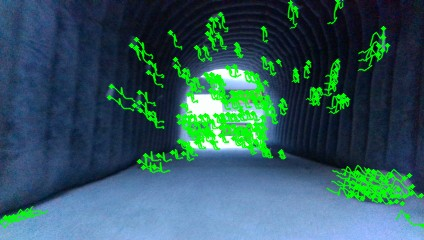
\includegraphics[width=\linewidth]{d7_30fps_lk_tracks.jpg}
    \caption{\code{30fps\_424x240}, frame 150.}\end{subfigure}\hfill
  \begin{subfigure}{0.58\linewidth}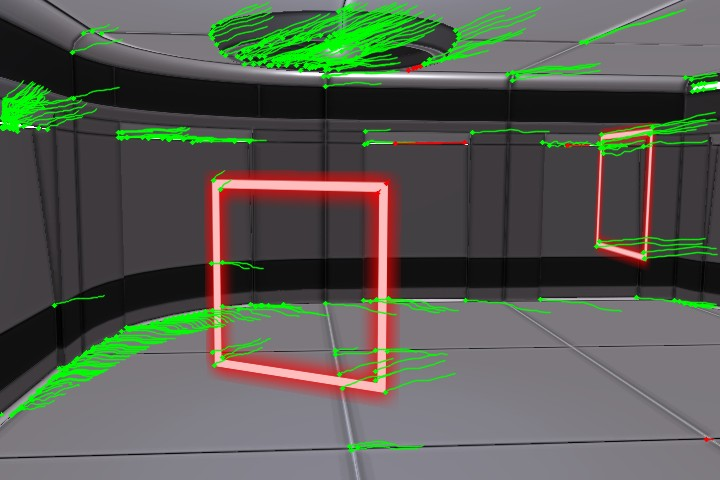
\includegraphics[width=\linewidth]{d7_smooth_lk_tracks.jpg}
    \caption{\code{smooth-trajectory}, frame 150.}\end{subfigure}
  \caption{Harris + LK feature tracks (last 20 frames of every track, green; RANSAC outliers red).}
  \label{fig:lk}
\end{figure}

\paragraph{Assumptions of the LK tracker.}
\begin{enumerate}
  \item \textbf{Brightness constancy:} a feature keeps the same intensity between
    frames, $I(x+\delta x, y+\delta y, t+\delta t)=I(x,y,t)$; linearising gives the optical
    flow constraint $I_x u + I_y v + I_t = 0$.
  \item \textbf{Small motion:} the displacement is small enough for that first-order
    Taylor expansion to hold (the image pyramid extends this to larger motions, coarse to
    fine).
  \item \textbf{Spatial coherence:} all pixels in the window around a feature move with
    the same (translational) flow, which gives an over-determined system solved by least
    squares. It is well conditioned only if the $2\times2$ structure tensor
    $\sum\nabla I\nabla I^\top$ has two large eigenvalues -- exactly what the Harris
    corner detector selects, which is why Harris corners and LK go together.
\end{enumerate}

\paragraph{Comparison with the descriptor-based methods.}
Harris+LK has the highest inlier ratio on both datasets (99.7\,\% and 95.5\,\%) and is
among the fastest (3.0 and 5.9\,ms per pair: no descriptors, the search is local, and the
corners of the previous frame are reused). Its number of inliers (552 and 255) is
comparable to ORB/FAST+BRIEF. The reason is that LK searches for each feature only around
its previous position, so it cannot produce the far-away ambiguous matches that a global
descriptor search can (e.g.\ between repeated gates or floor tiles), and the inlier-only
tracking removes bad points. On the other hand, LK only works under its assumptions: it
needs small inter-frame motion and constant brightness, it slowly drifts, and it cannot
match two unrelated views. It would fail completely on the box pair of
Deliverable~6.a and cannot be used for loop closure or re-localisation, where
descriptors are needed. In the per-frame plots (Fig.~\ref{fig:perframe}) LK is also the
most stable curve, while the descriptor methods have dips at fast rotations.

\subsection{Deliverable 8 (optional) -- Farneback dense optical flow}

The node in \code{self\_flow.cpp} computes the dense flow between consecutive grayscale
frames with Farneback's polynomial-expansion method~\cite{farneback2003flow}
(\code{calcOpticalFlowFarneback}; pyramid scale 0.5, 3 levels, $15\times15$ window, 3 iterations,
polynomial neighbourhood 5, $\sigma=1.2$) and shows, side by side, the frame with the
flow vectors on a 16-pixel grid and a colour-coded flow field (hue = direction,
brightness = magnitude, saturated at 10\,px). We ran it on both datasets
(\code{roslaunch lab\_5} \code{self\_flow.launch}); Fig.~\ref{fig:flow} shows one frame, and
\code{video/d8\_farneback\_flow\_*.mp4} the full sequences. During the rotation in
Fig.~\ref{fig:flow} the flow is nearly uniform (one colour) on the far walls and much
larger on the nearby door frame on the right, as expected from parallax. Textureless
regions (uniform walls, floor) get unreliable, near-zero flow, since no method can
estimate motion where the image has no gradient (aperture problem).

\begin{figure}[h]
  \centering
  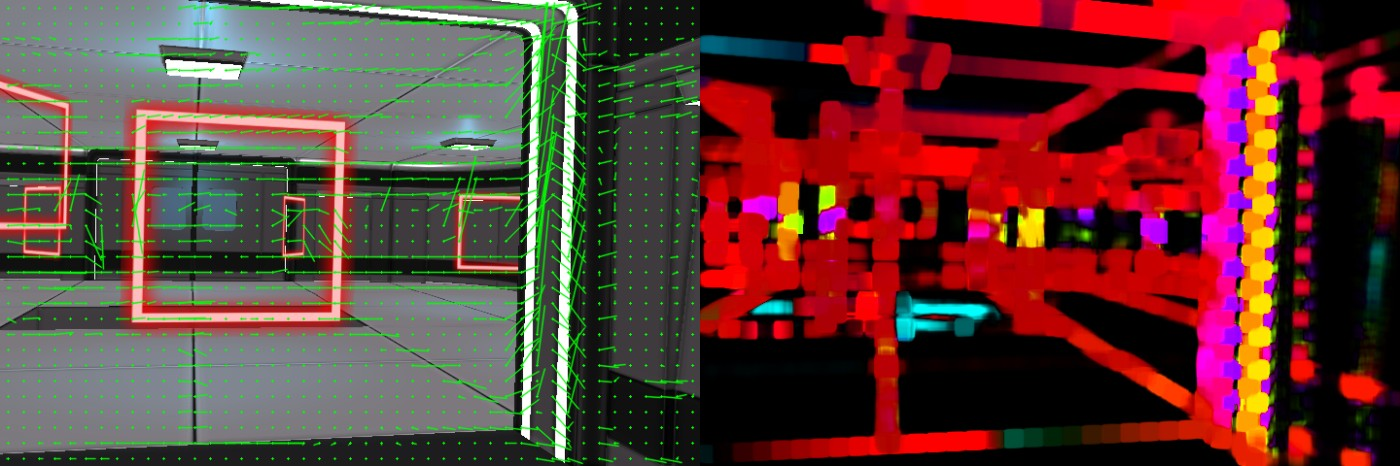
\includegraphics[width=\linewidth]{d8_smooth_farneback.jpg}\\[0.4em]
  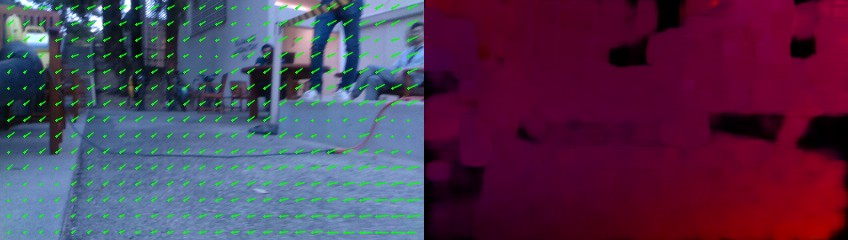
\includegraphics[width=0.75\linewidth]{d8_30fps_farneback.jpg}
  \caption{Farneback dense optical flow. Left: frame with flow vectors ($2\times$
    scaled); right: colour-coded flow. Top: simulated dataset, bottom: real dataset.}
  \label{fig:flow}
\end{figure}

\subsection{Reproducing the results}
\begin{verbatim}
bash scripts/build_workspace.sh            # opencv3_catkin + lab_5
source ~/vnav-builds/lab5_ws/devel/setup.bash && roscore &
roslaunch lab_5 two_frames_tracking.launch descriptor:=SIFT   # interactive D3-D5
python3 scripts/run_experiments.py pair    # D3-D6a  -> results/d6a_pair/
python3 scripts/run_experiments.py video --frames-for SIFT LK # D6b, D7
bash scripts/run_flow.sh 30fps; bash scripts/run_flow.sh smooth   # D8
python3 scripts/make_figures.py            # report/figures/ + table rows
bash scripts/make_videos.sh; bash scripts/build_report.sh
\end{verbatim}


\bibliographystyle{unsrtnat}
\bibliography{references}

\end{document}
